\documentclass[11pt]{article}
\usepackage[margin=2cm]{geometry}
\usepackage{graphicx}
\usepackage{amsmath,amssymb}
\setlength{\parindent}{0pt}\setlength{\parskip}{5pt}
\newcommand{\code}[1]{\texttt{#1}}
\begin{document}
\begin{center}{\Large\bfseries Common figures --- Notes for the Defense}\\[2pt]
The task-level figures: they describe the problem, not a model, so they come BEFORE any per-model result and are shared by every whole-body package.\end{center}
\vspace{4pt}
\section*{Figure 1 --- The T-arc spawn envelope and the robot start pose}
\begin{center}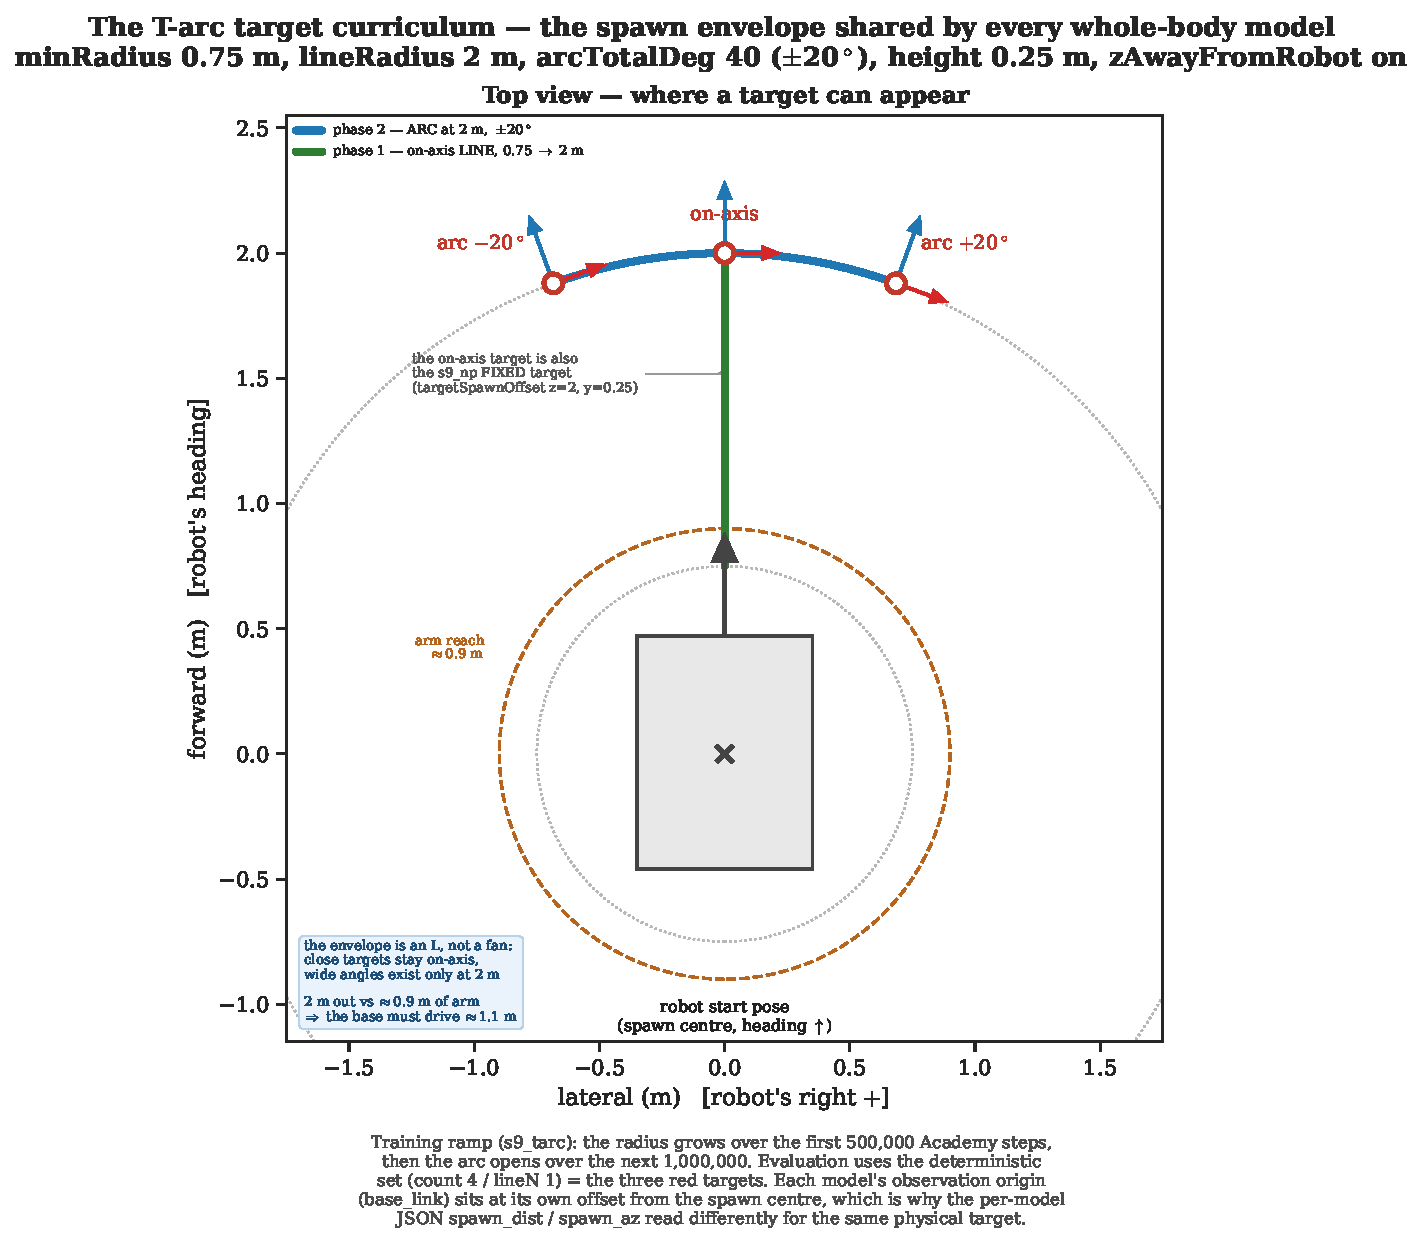
\includegraphics[width=0.72\textwidth,height=0.62\textheight,keepaspectratio]{target_spawn_area.pdf}\end{center}
\textbf{What it shows.} Where a target can be created, relative to the robot's start pose, seen from above. The green segment is the on-axis line (0.75$\to$2 m), the blue arc is the far arc at 2 m spanning $\pm20^\circ$, and the three red circles are the deterministic evaluation targets, drawn with their frame axes. The target always sits 0.25 m above the base.

\textbf{How to read it.} The envelope is an \textbf{L}, not a filled fan: the curriculum first pushes the target out along the axis, and only then opens the angle at the far radius, so a close target is never also strongly off-axis. The dashed circle carries the reason this is a whole-body problem at all: the target is at 2 m while the arm reaches about 0.9 m, so roughly 1.1 m has to be covered by driving the base.

\textbf{Say this.} ``Every whole-body model is trained and evaluated on this same envelope --- 2 m out, $\pm$20\textdegree, 25 cm up --- so the comparisons that follow are on identical targets.''

\textbf{If asked.} \emph{Why not sample the whole fan?} --- because close-and-wide targets would be behind the robot's shoulder, a qualitatively different (and much harder) problem than the one this stage is about. \emph{Why do the JSON spawn distances differ per model?} --- they are measured from each robot's own \texttt{base\_link}, which sits at a different offset from the spawn centre; the physical geometry is the same, and that was verified by fitting a circle to the logged target positions.
\clearpage
\section*{Figure 2 --- What \emph{confondu} means: the two frames and the two errors}
\begin{center}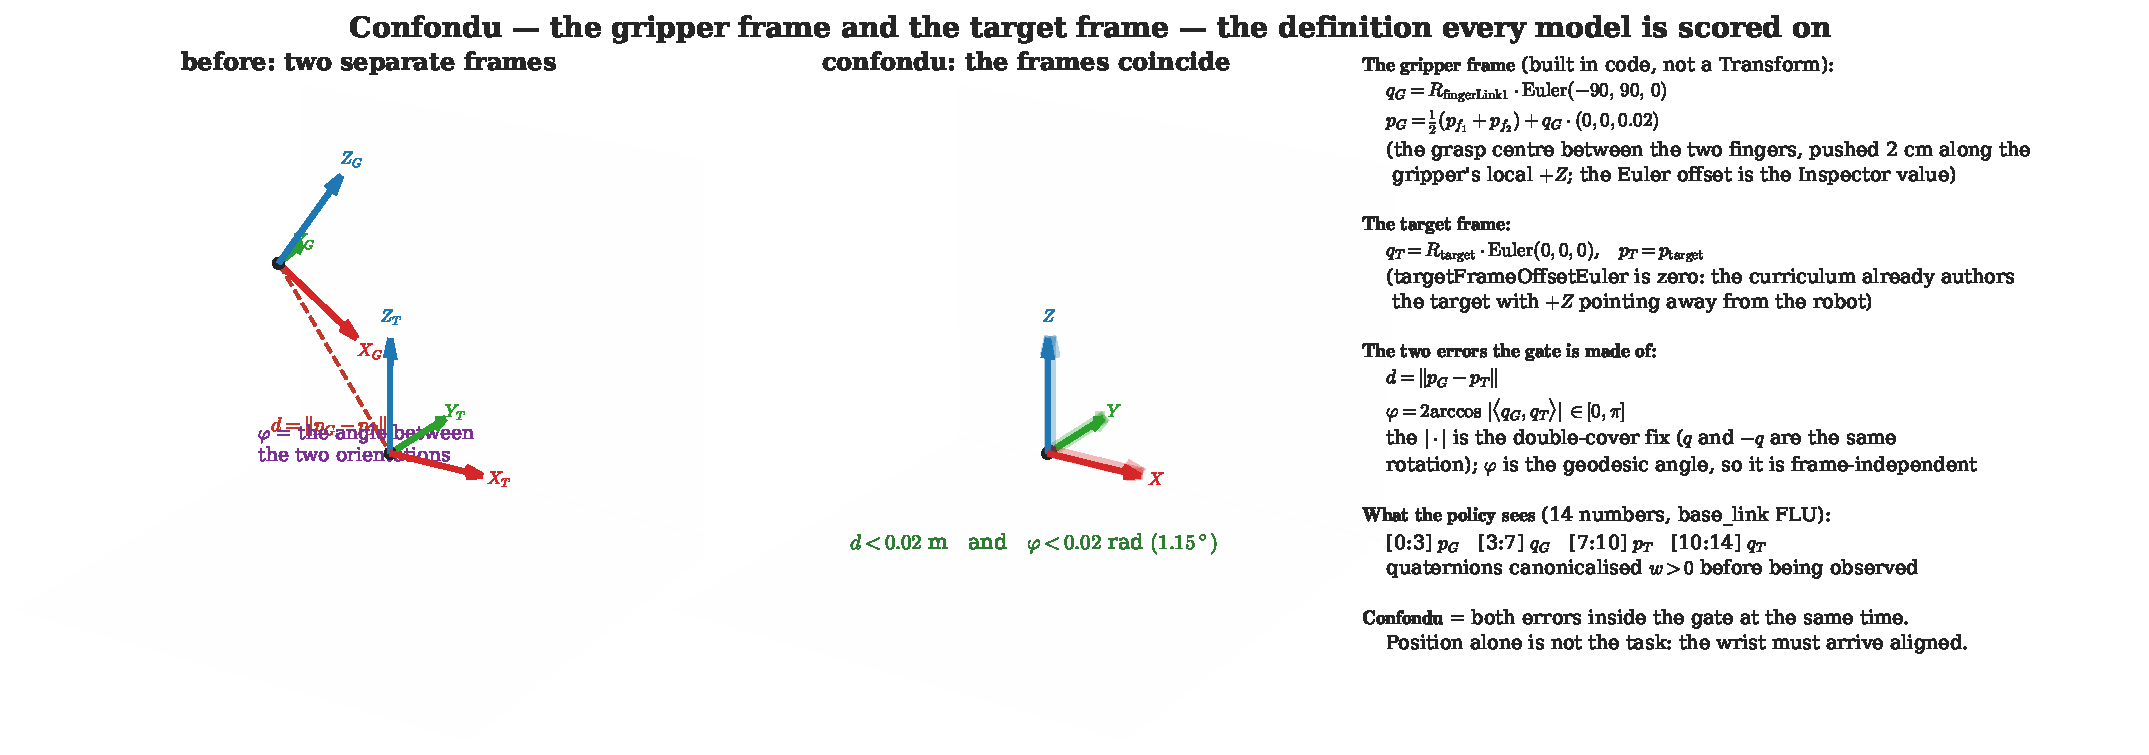
\includegraphics[width=0.99\textwidth,height=0.46\textheight,keepaspectratio]{frames_confondu.pdf}\end{center}
\textbf{What it shows.} The gripper frame and the target frame as RGB triads (X red, Y green, Z blue --- the same convention as the in-scene axis renderer), how each one is constructed from the serialized offsets, and the two error measures the success gate is made of.

\textbf{How to read it.} The left panel is a normal mid-episode state: the origins are $d$ apart and the orientations differ by $\varphi$. The middle panel is the goal: the triads sit on top of each other. The gripper frame is \emph{computed}, not a Transform in the scene --- it is finger link 1's rotation times the Euler offset $(-90,90,0)$, and the origin is the grasp centre pushed 2 cm forward.

\textbf{Say this.} ``The task is frame coincidence, not reaching: the gripper must arrive at the target's position \emph{and} in the target's orientation --- under 2~cm and 1.15\textdegree{} at the same time.''

\textbf{If asked.} \emph{Why the absolute value in $\varphi$?} --- a quaternion and its negative are the same rotation; without $|\cdot|$ the metric reports the long way round (e.g. 330\textdegree{} instead of 30\textdegree). \emph{Why is the gripper frame not just the finger's transform?} --- the finger link's authored axes do not match the target's convention; the Euler offset is what makes the two frames comparable, and getting it wrong makes the gate unreachable without any error message.
\clearpage
\end{document}
